\chapter{Introduction}
\label{chap:introduction}

    In this report we will discuss our security analysis of a Wi-Fi extender produced by Aigital (Figure~\ref{fig:router}).
    
    \begin{figure}[H]
        \centering
        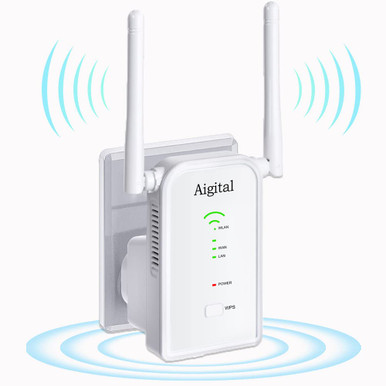
\includegraphics[width=0.5\textwidth]{../imgs/1.1-extender.jpg}
        \caption{Aigital Wi-Fi Extender}
        \label{fig:router}
    \end{figure}

    \section{Device Informations}
        The Aigital Wi-Fi Extender is a device that allows to extend the coverage of a Wi-Fi network.
        \\
        It was bought in 2019 and is still available for purchase on Amazon\footnote{\url{https://amazon.it/dp/B0DR7ZT2CS}} and it is sold at a price of around 20 euros.
%        \begin{figure}[H]
%            \centering
%            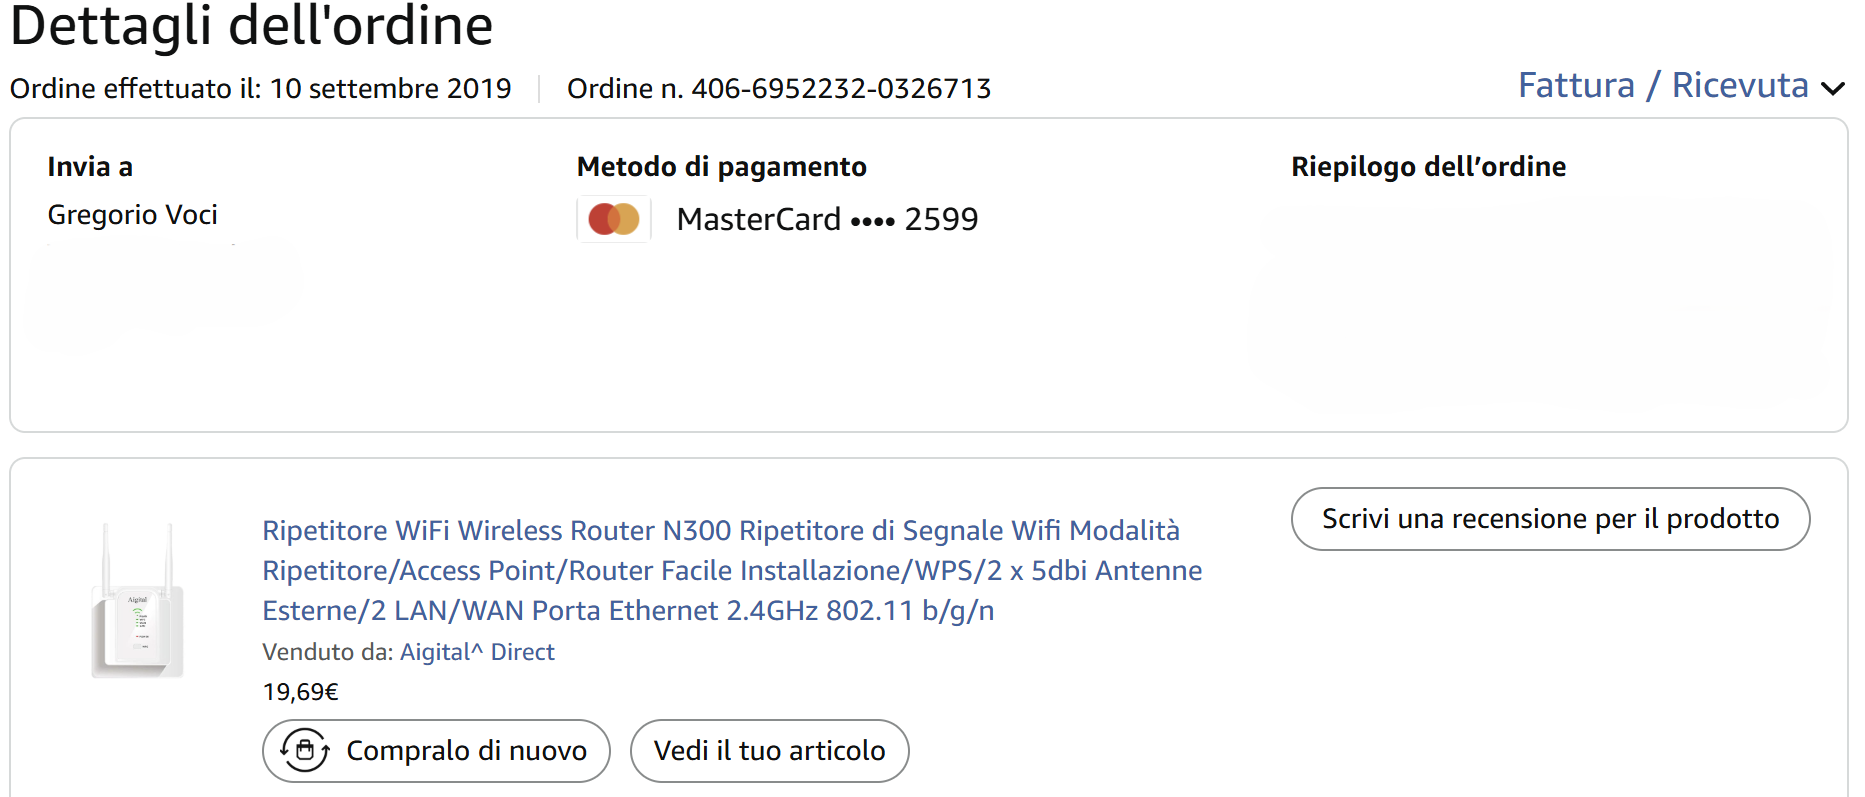
\includegraphics[width=1\textwidth]{../imgs/ordine.png}
%            \caption{Order details (sensible information redacted)}
%        \end{figure}
%        \newpage
        \\
        The device has a web interface for configuration and management, which is accessible through the local network on 192.168.10.253 (Figure~\ref{fig:web_interface}).
        
        \begin{figure}[H]
            \centering
            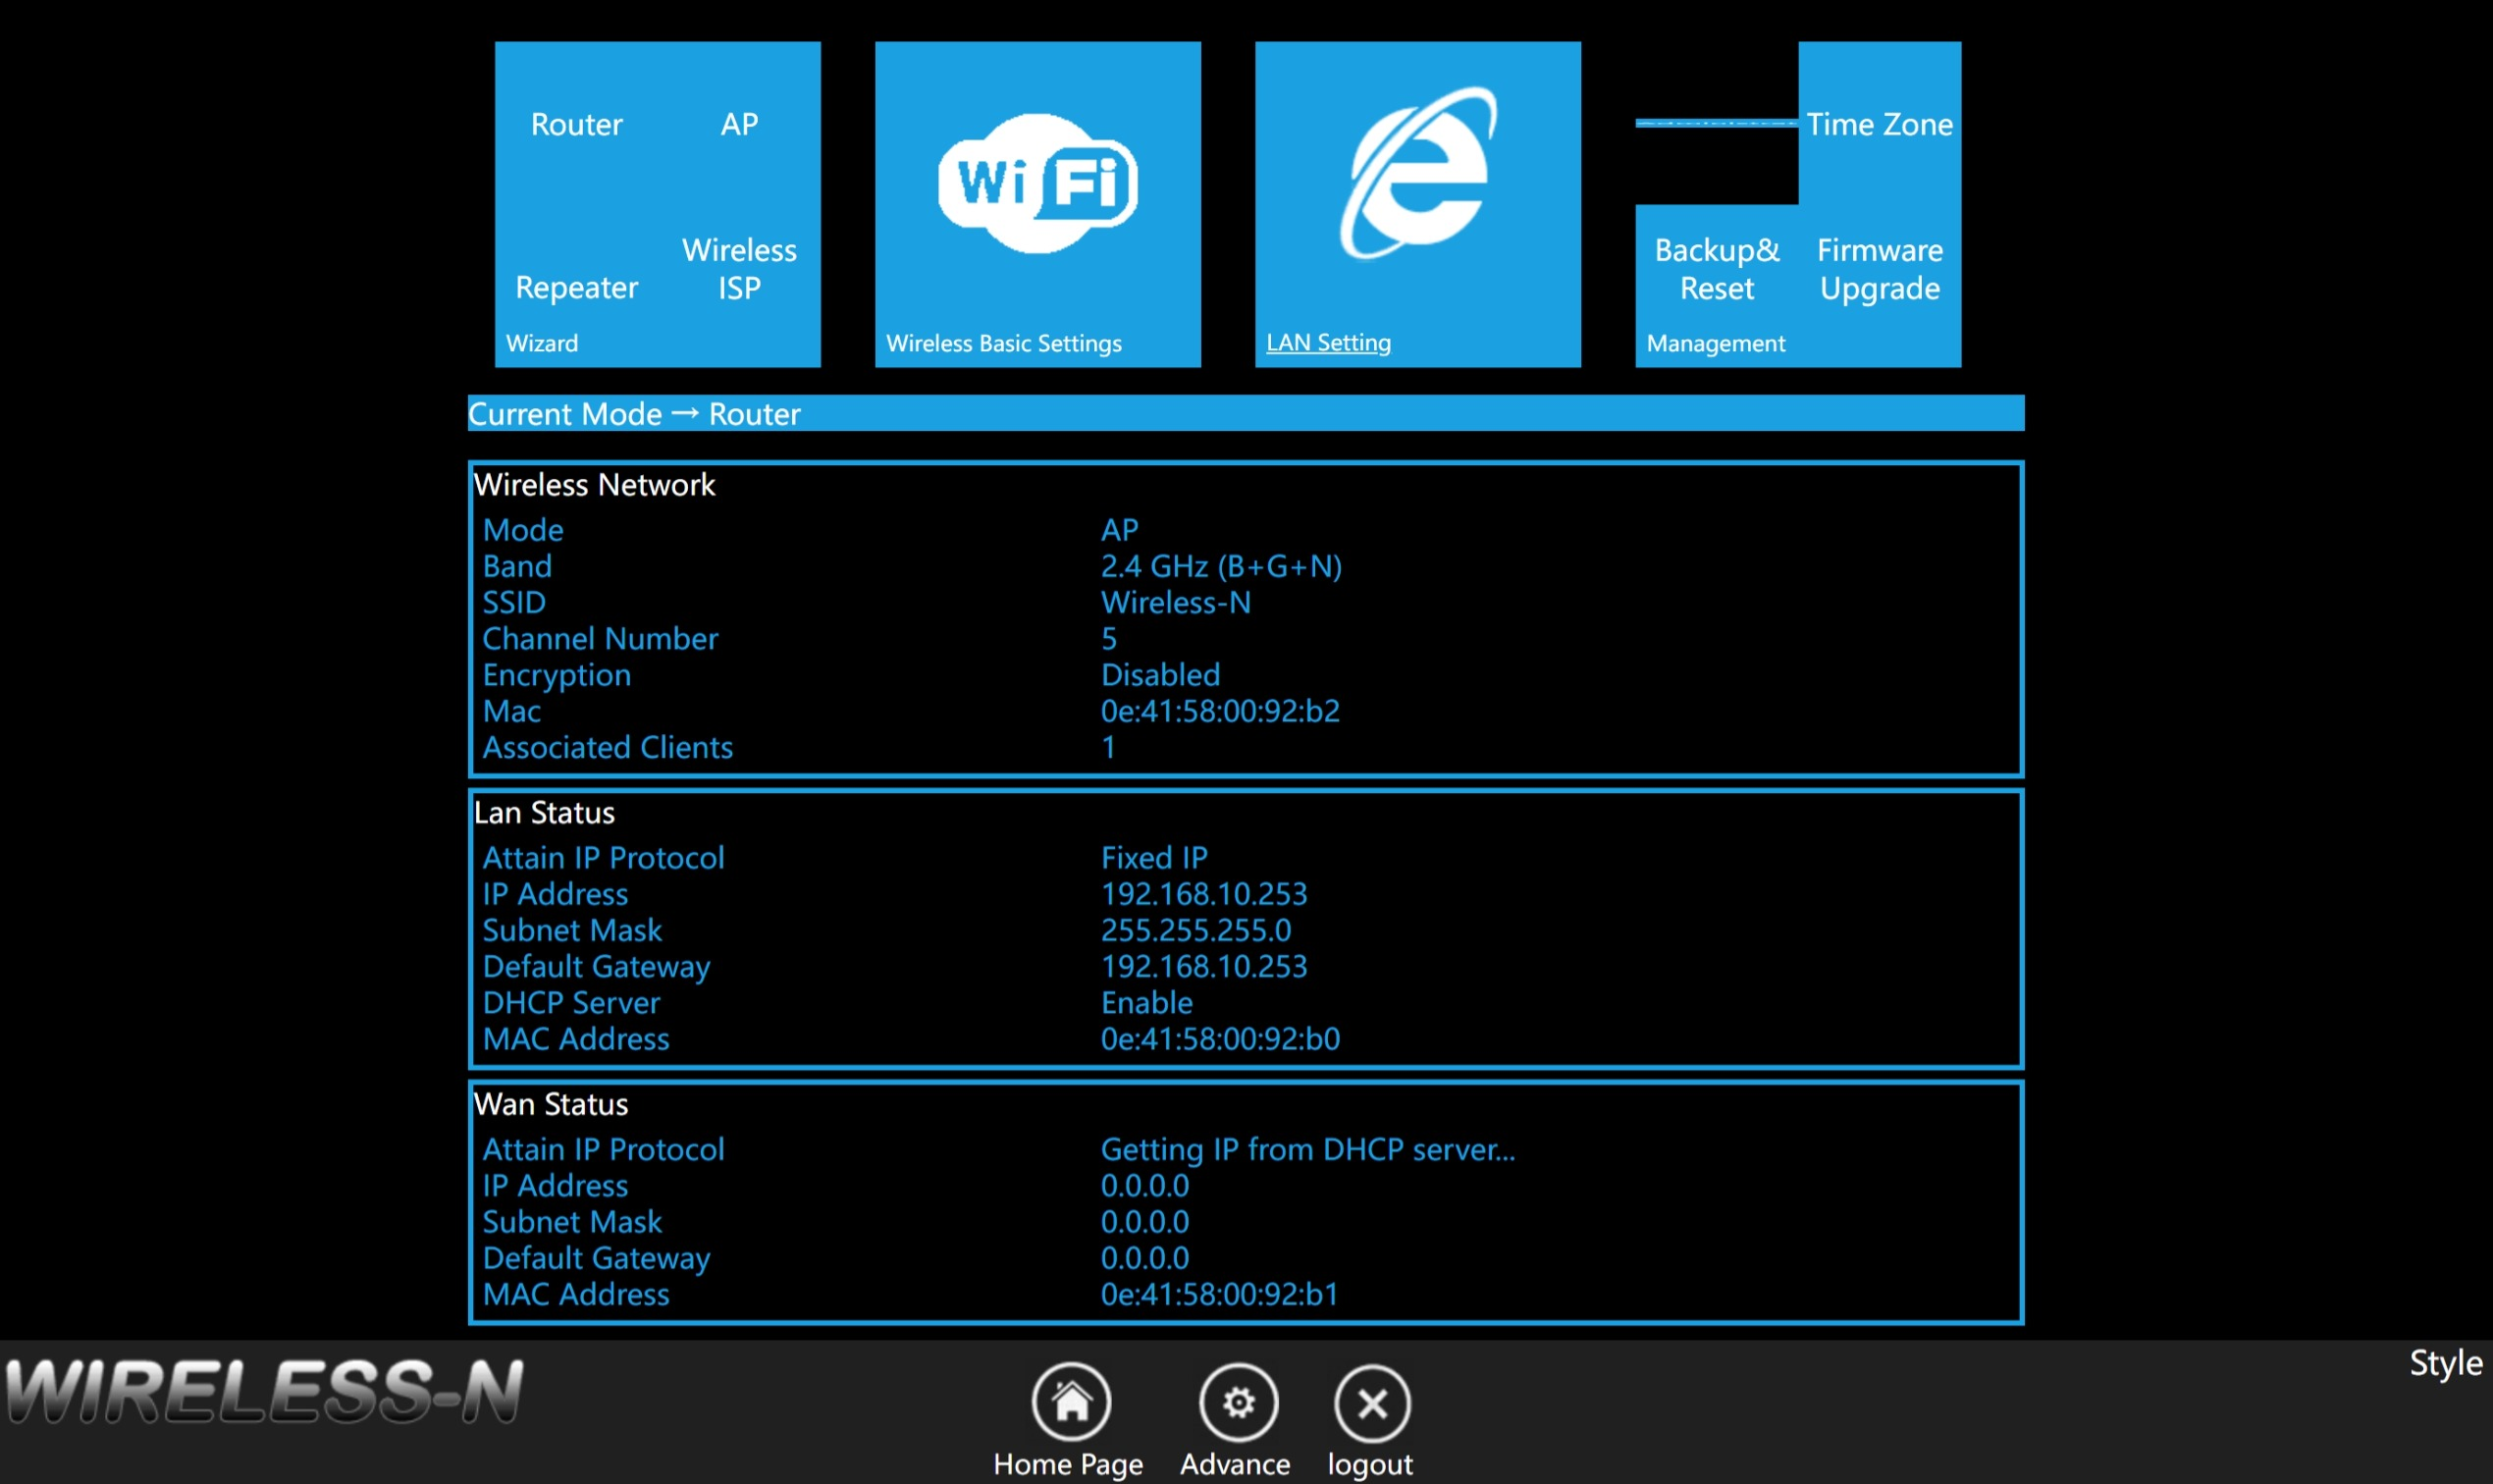
\includegraphics[width=0.8\textwidth]{../imgs/1.2-web_page.jpeg}
            \caption{Web interface}
            \label{fig:web_interface}
        \end{figure}

    \section{Objectives}
        As we will see in the next sections, our main goal was to exploit the CVE-2023-30403\cite{CVE-2023-30403}, CVE-2023-30404\cite{CVE-2023-30404} and CVE-2023-30405\cite{CVE-2023-30405} vulnerabilities, which allow for login by-pass, remote code execution and cross-site scripting respectively. 
        \\
        We also wanted to analyze the firmware of the device, in order to find other potential vulnerabilities and to understand how the device works.
        \\
        Finally, we wanted to patch the CVEs compiling a custom firmware.
    \section{Tools Used}
        We used a variety of tools for our analysis, including:
        \begin{itemize}
            \item A digital multimeter for individuating the pins of the UART interface;
            \item A USB-to-TTL adapter for analyzing the UART communication;
            \item A CH341A programmer with a soic clip for dumping the EEPROM with flashrom;
            \item Binwalk for firmware analysis;
            \item Ghidra and Cutter for reverse engineering the firmware;
            \item A custom script for patching the firmware.
        \end{itemize}
        All of our codes are available on our GitHub repository\footnote{\url{https://github.com/Gory-git/progetto_IoT}}.
    \section{Issues Encountered}
        We feel it is important to note in advance that at a certain point in the project, we encountered some issues with the access point’s hardware that took up a significant amount of our time. 
        \\
        Specifically, while attempting to open a reverse shell on the device, we uploaded a binary to it whose size exceeded the available memory, causing the device to brick. To reflash the working binary, we desoldered the EEPROM. Unfortunately, we weren’t careful enough and broke a trace on the PCB, as shown in the Figure~\ref{fig:broken_trace}.  

        \begin{figure}[H]
            \centering
            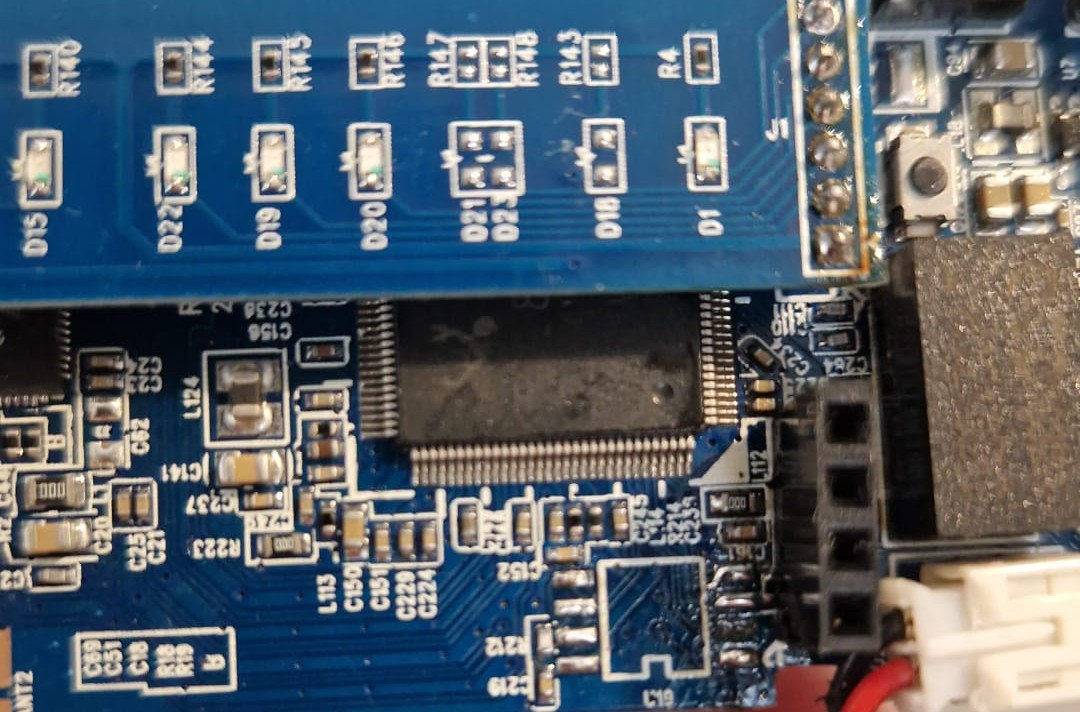
\includegraphics[width=0.8\textwidth]{../imgs/1.3-pista-rotta.jpeg}
            \caption{Broken trace}
            \label{fig:broken_trace}
        \end{figure}

        With the help of a friend of ours who is an electrical engineering student, we repaired the previously broken circuit trace and, to avoid further problems, installed a socket on the PCB so that the EEPROM can be easily inserted and removed for future testing (Figures~\ref{fig:rep1}, ~\ref{fig:rep2}, ~\ref{fig:rep3}).

        \begin{figure}[H]
            \centering
            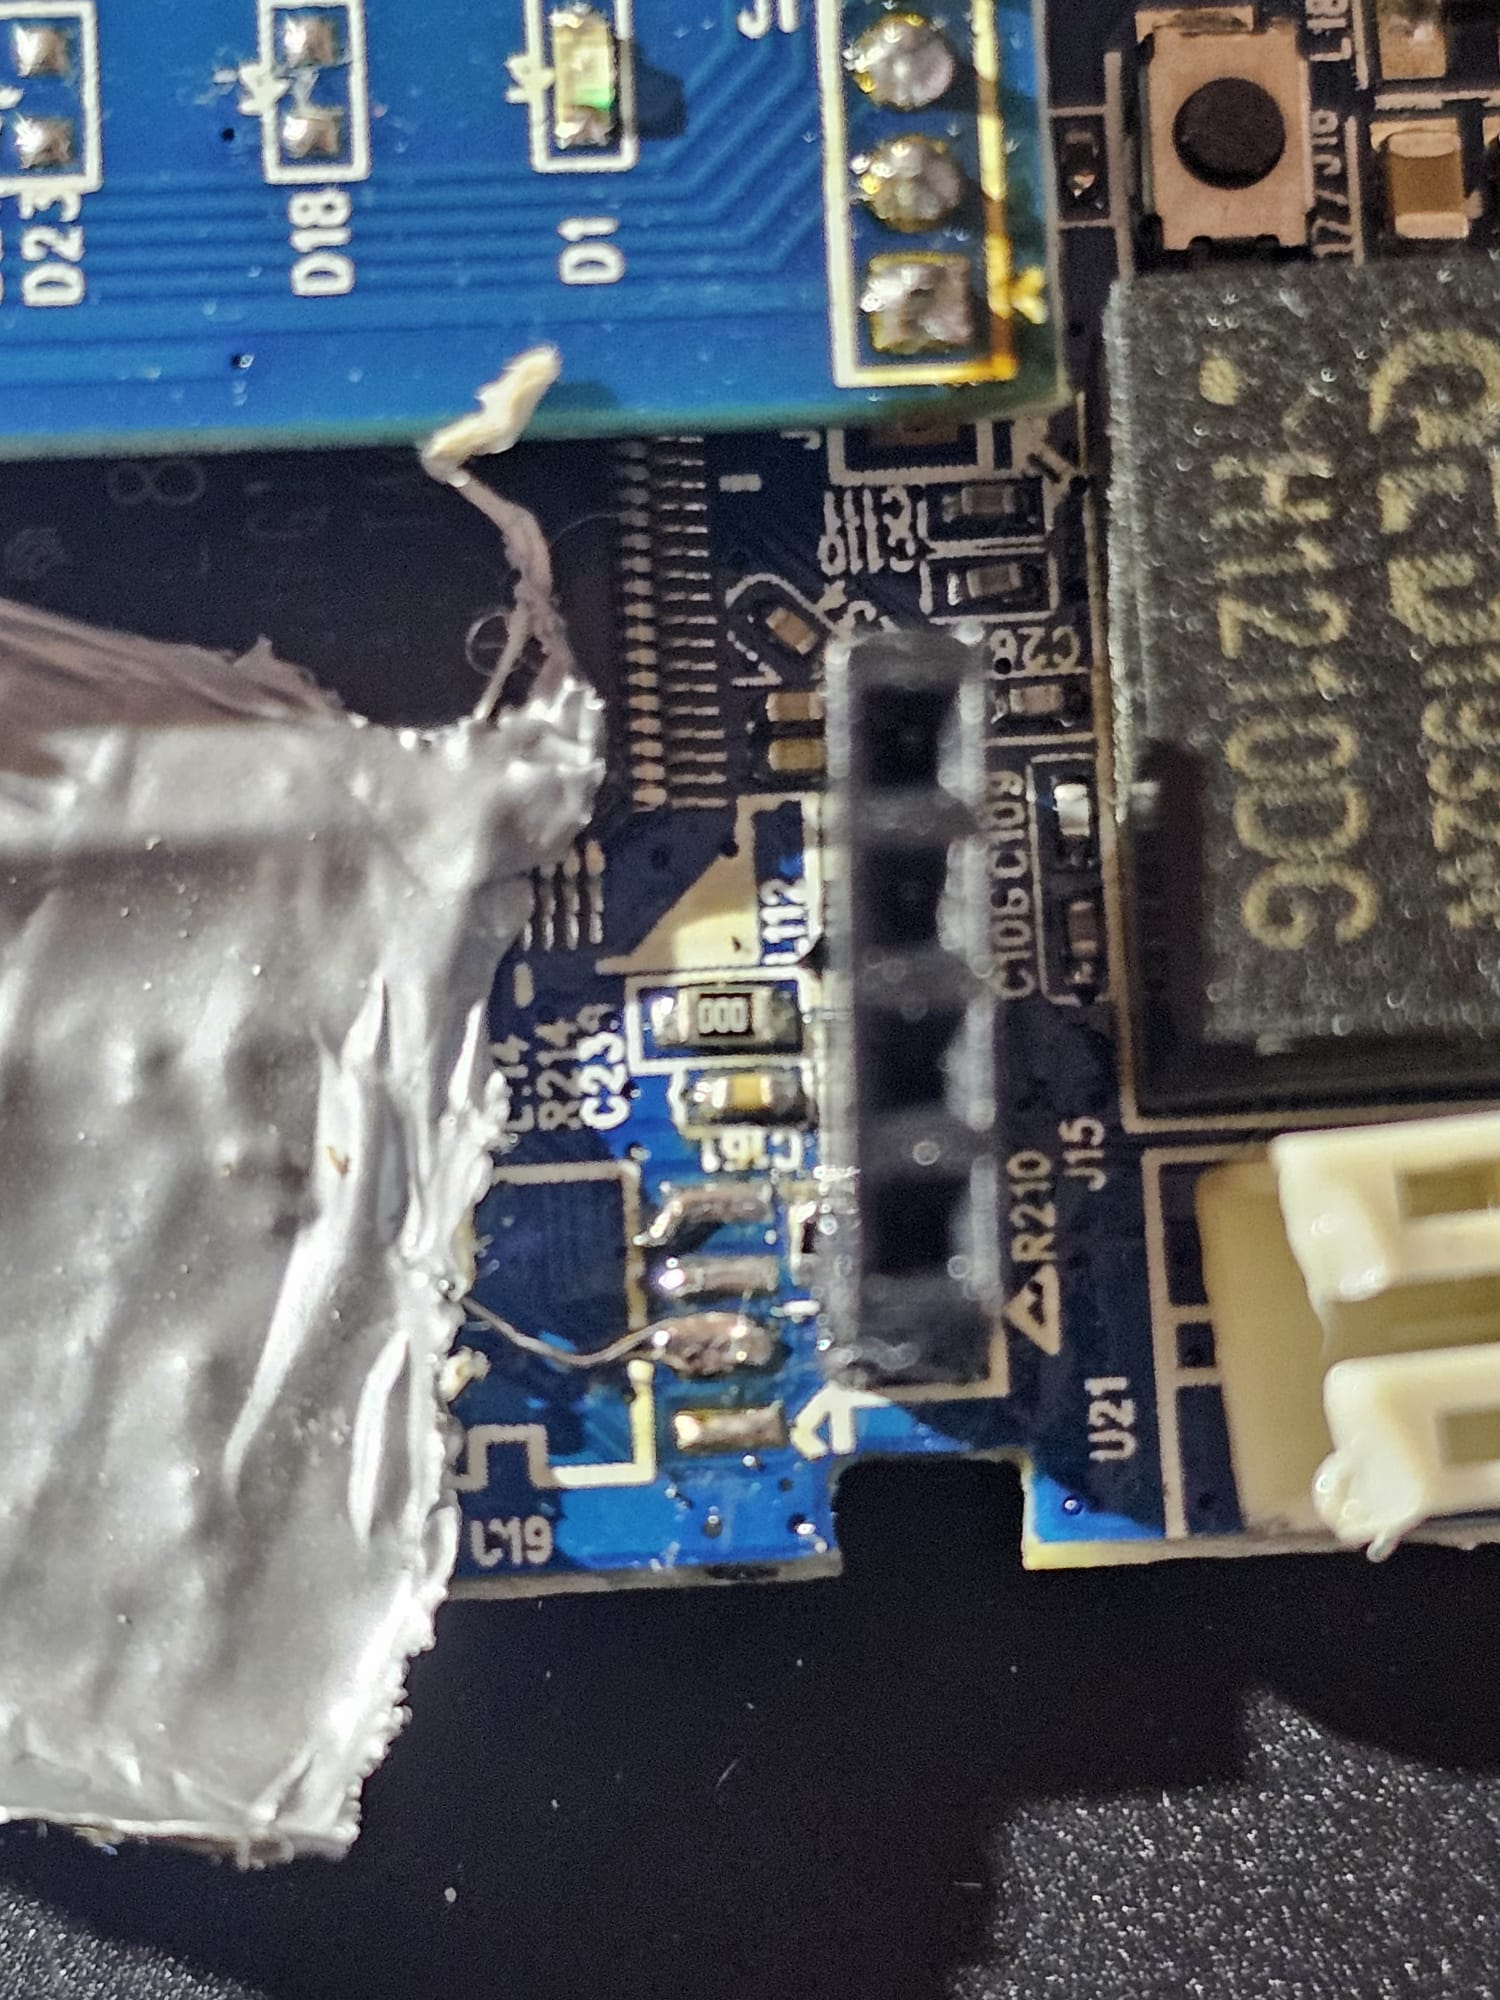
\includegraphics[width=0.8\textwidth]{../imgs/1.4-riparazione-1.jpeg}
            \caption{Reparation process 1}
            \label{fig:rep1}
        \end{figure}
        \begin{figure}[H]
            \centering
            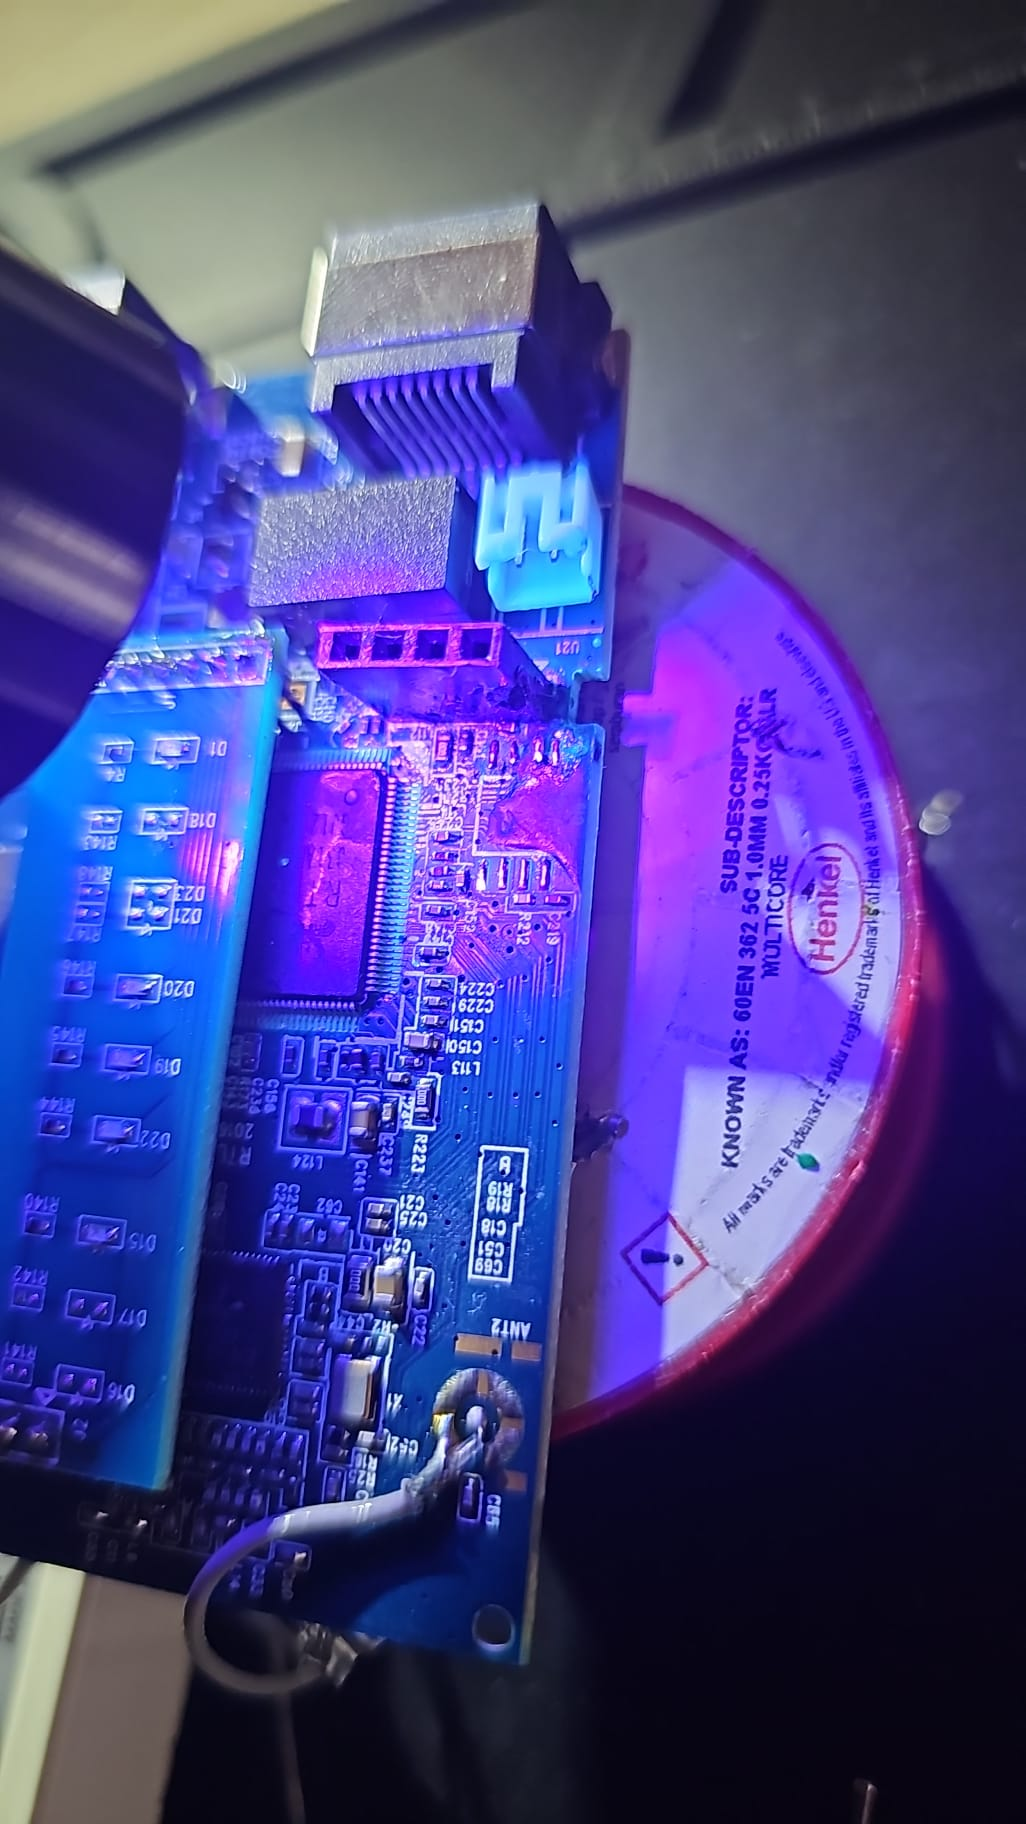
\includegraphics[width=0.8\textwidth]{../imgs/1.5-riparazione-2.jpeg}
            \caption{Reparation process 2}
            \label{fig:rep2}
        \end{figure}
        \begin{figure}[H]
            \centering
            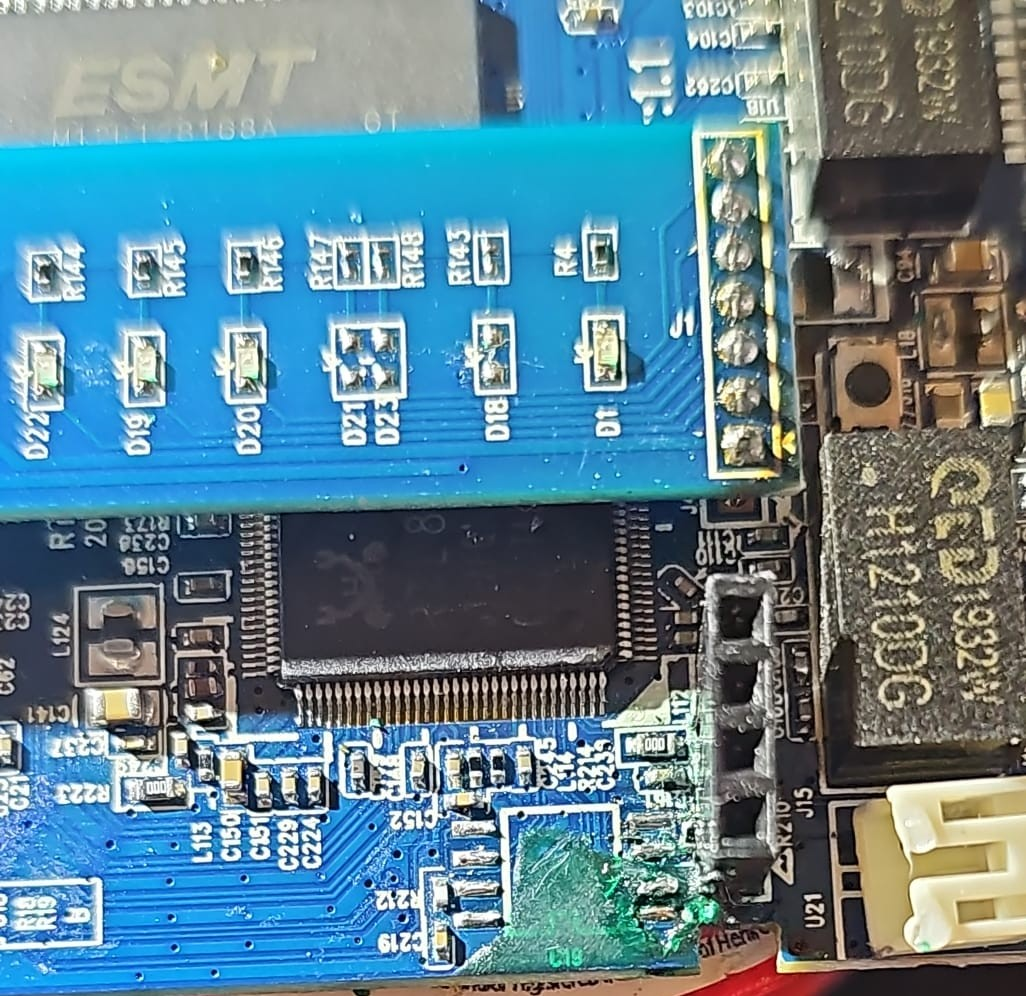
\includegraphics[width=0.8\textwidth]{../imgs/1.6-riparazione-3.jpeg}
            \caption{Reparation process 3}
            \label{fig:rep3}
        \end{figure}
        
        To top it all off, though, we broke one of the chip’s pins while repeatedly inserting and removing the EEPROM (Figure~\ref{fig:brokenEeprom}). 

        \begin{figure}[H]
            \centering
            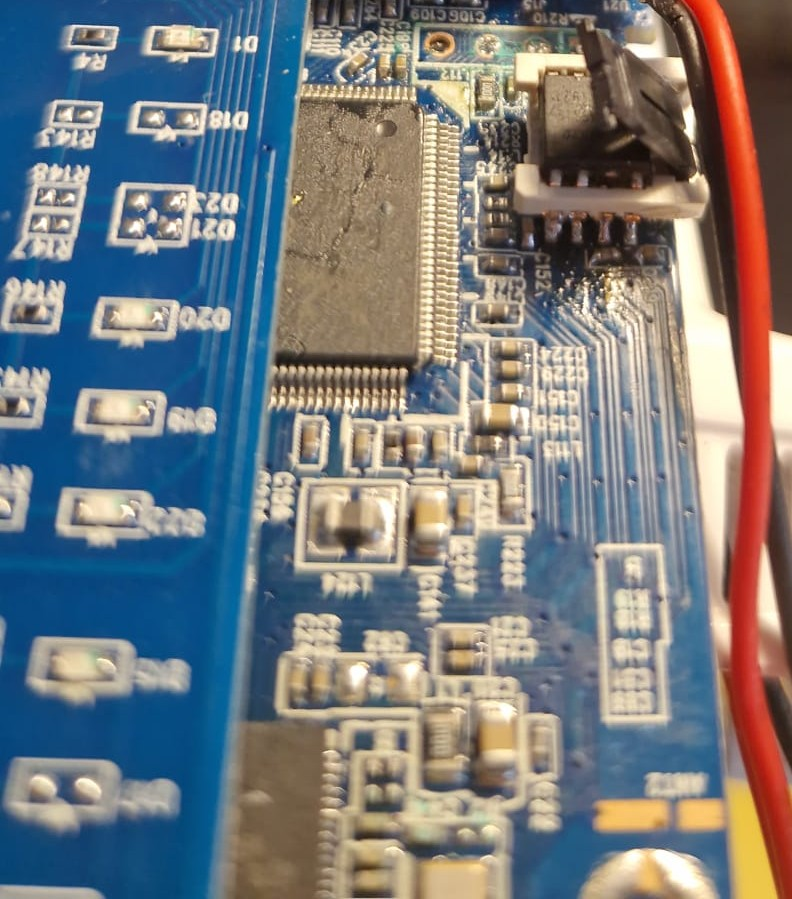
\includegraphics[width=0.8\textwidth]{../imgs/1.7-eeprom-rotta.jpeg}
            \caption{Broken EEPROM}
            \label{fig:brokenEeprom}
        \end{figure}
        
        To avoid wasting any more time fixing this problem, we continued with the project by fully emulating the firmware, including the web server, using Firmadyne. Further details are available in the section~\ref{sec:firmware emulation}.

        